\chapter{Results}
\label{ch:results}

% TODO results: make numbers in table captions pretty ($$), and make at\% into at.\% in tables


% intro to results
This chapter presents the results of the thesis.
The results are divided into three parts: an initial qualitative analysis of the spectra, followed by the performance parameters of the setup and acquisition parameters, and finally the quantification results.
As seen in the SE images presented in \cref{method:materials}, the areas chosen for the analysis are homogeneous and relatively clean.
Scratched areas on the GaSb specimen are shown in \cref{fig:SE_images:GaSb} panel (b), where some spectra were acquired, but not included in the results of this thesis.
% DONE discuss: the scratched areas behaved as expected, yielding poorer results than the homogeneous areas. ISO etc.



% 1 qualitative analysis
\section{Qualitative analysis}
\label{results:qualitative_analysis}

Here, an overview of the spectra is presented, where some characteristics and artifacts are identified.
General plots of the spectra are given in \cref{fig:results:overviewGaSb_withArtifacts,fig:results:GaSb_voltages,fig:results:GaAs_voltages}.

% figures/results/spectrum_overview.pdf
% TODO results: make (b) green? To distinguish from (a)
\begin{figure}[hbtp]
    \centering
    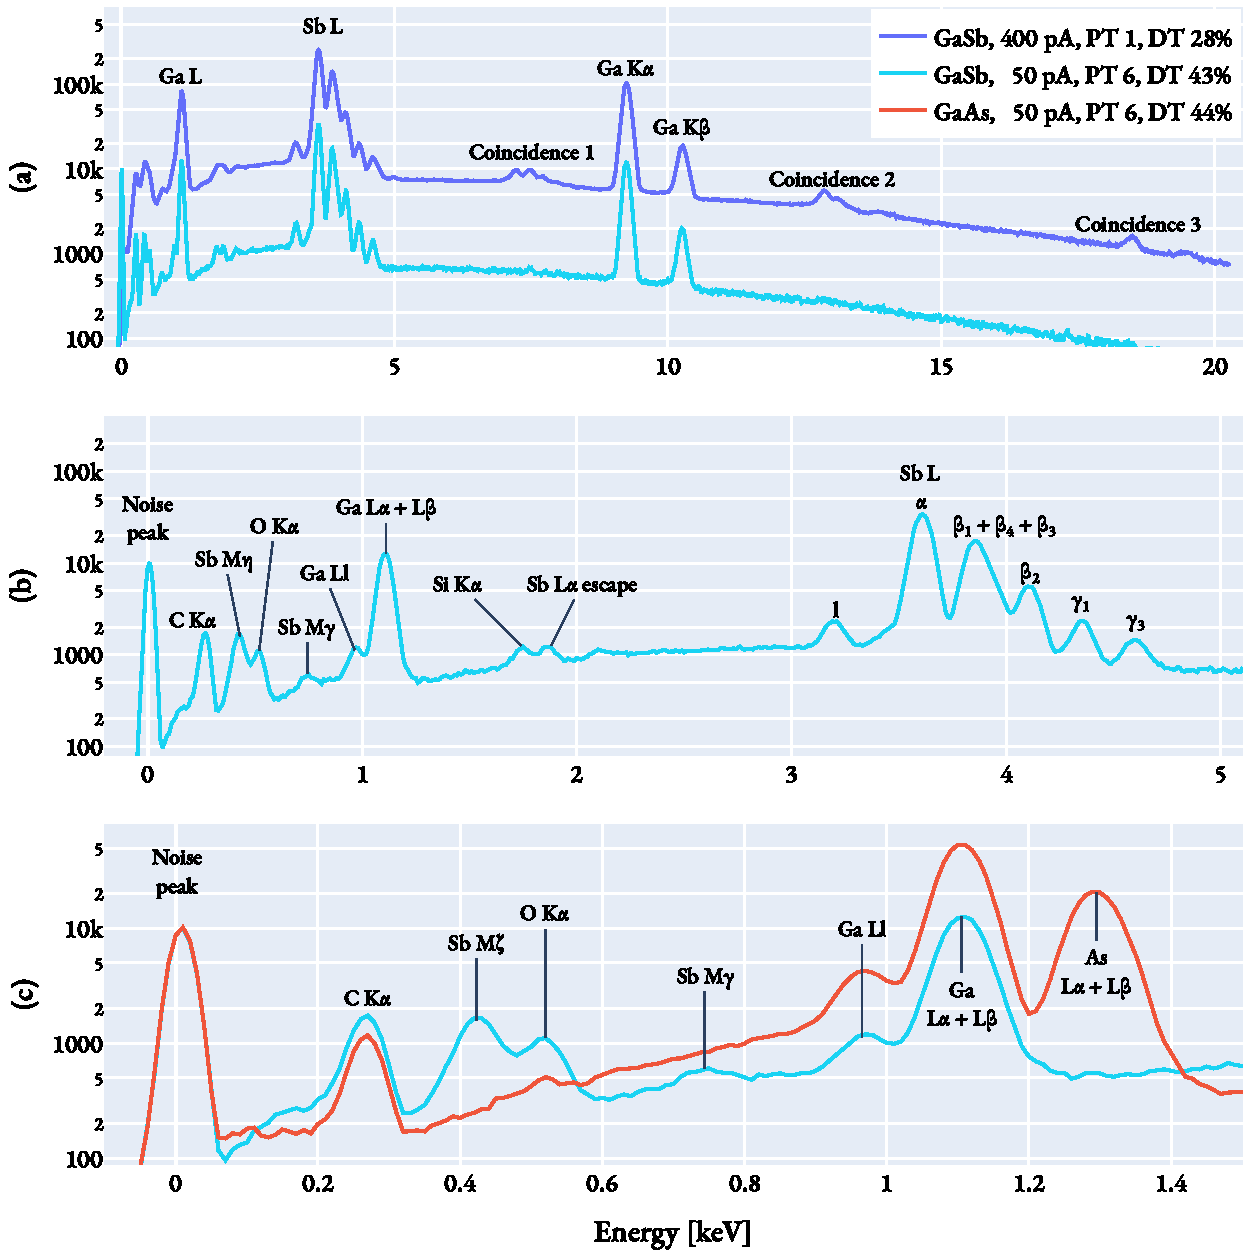
\includegraphics[width=0.99\linewidth]{figures/results/spectrum_overviews.pdf}
    \caption{
        Overview of the GaSb spectra.
        The blue line in panel (a) have lower resolution and more artifacts than the light blue line.
        The light blue line is plotted in panel (b) over a shorter energy range, and with peaks annotated.
        Panel (c) show the light blue line on an even shorter energy range, with the GaAs spectrum in red for reference.
        All three spectra are acquired with $30$ kV.
    }
    \label{fig:results:overviewGaSb_withArtifacts}
\end{figure}

% figures/results/GaAs_voltages.pdf
\begin{figure}[hbtp]
    \centering
    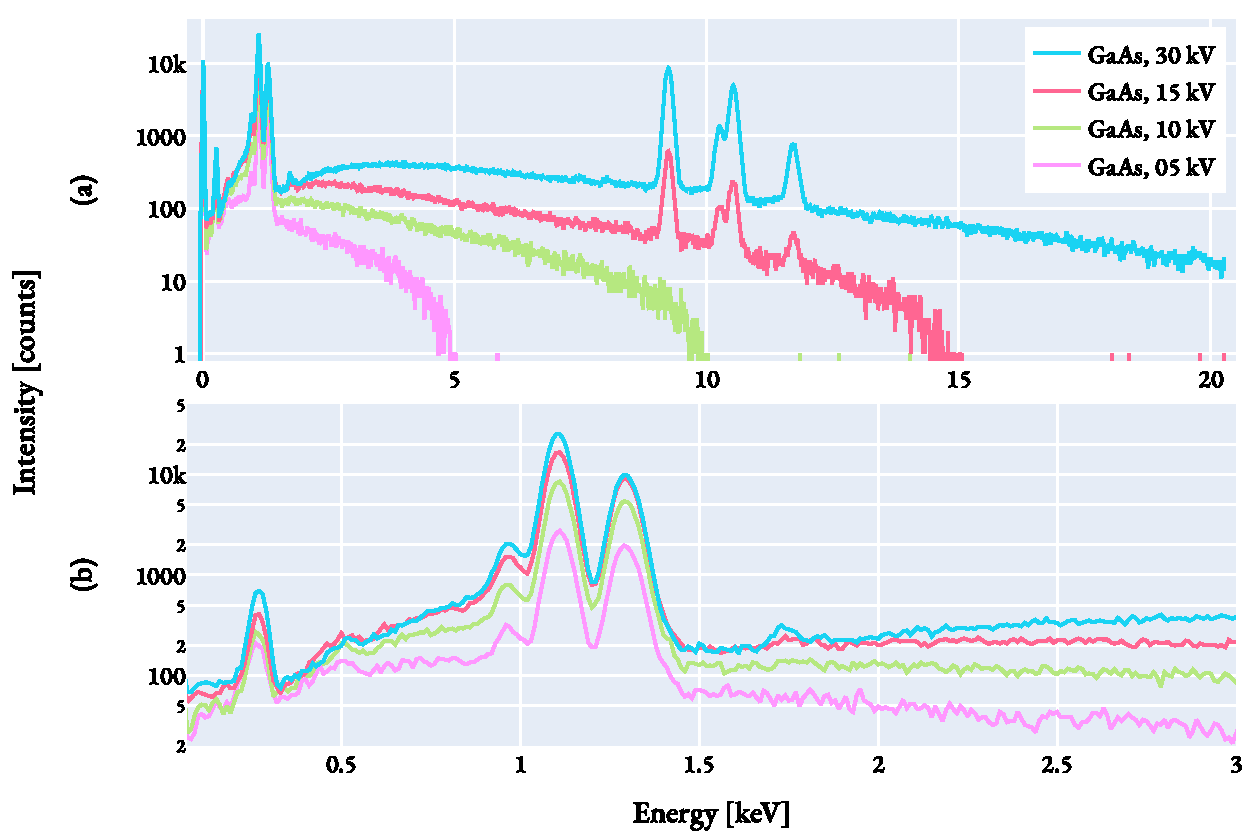
\includegraphics[width=0.85\linewidth]{figures/results/GaAs_voltages.pdf}
    \caption{
        Group (A), the GaAs voltage series.
        The figure gives an overview of the spectra, and show the effect of overvoltage.
        All four spectra have $i_b = 25$ pA and PT $6$.
    }
    \label{fig:results:GaAs_voltages}
\end{figure}

% figures/results/GaSb_voltages.pdf
\begin{figure}[hbtp]
    \centering
    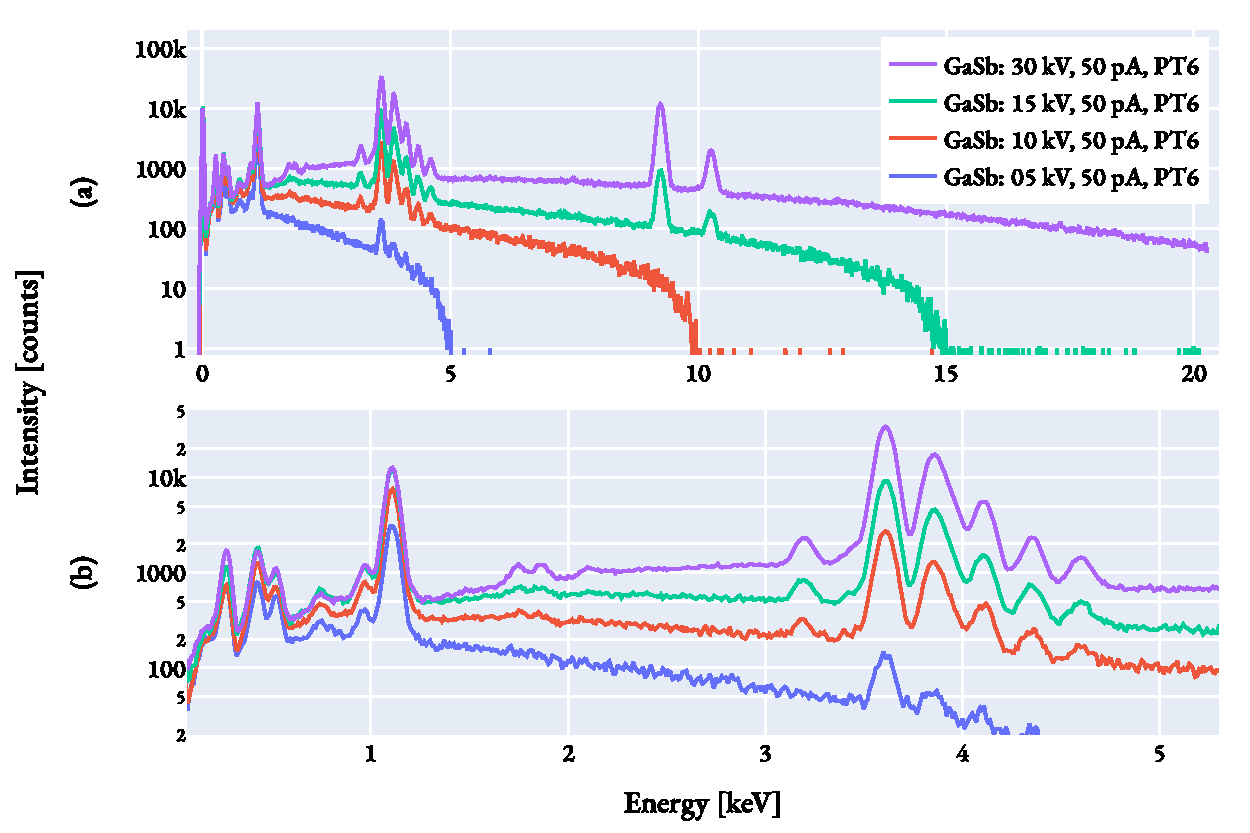
\includegraphics[width=0.85\linewidth]{figures/results/GaSb_voltages.pdf}
    \caption{
        Group (B), the GaSb voltage series.
        The figure serves the same purpose as \cref{fig:results:GaAs_voltages}, but for GaSb.
        % Additionally, an increased amount of coincidence counts compared to the GaAs spectra is visible in the tailing backgrounds, especially at 15 kV.
        The tailing background is the vertical lines above $E_0$.
        All four spectra have $i_b = 50$ pA and PT $6$.
    }
    \label{fig:results:GaSb_voltages}
\end{figure}




The lines given in \cref{tab:theory:lineEnergies} for Ga, As, and Sb have been identified in the spectra.
All spectra also had a peak at C K$\alpha$.
% DONE Ton: discus this C_Ka artifact, origin, in discussions
% DONE Ton: No other common peaks like Fe, or Si from setup?
The GaSb spectra included a well-defined O K$\alpha$ peak, while the GaAs spectra had barely any signal from the O K$\alpha$ line.
% DONE discuss: the O Ka peak might also be a Sb M-line, but I have not found the energy of the Sb M-lines.
As annotated in \cref{fig:results:overviewGaSb_withArtifacts}, the GaSb spectra also included two Sb M-signals: $\zeta$ and $\gamma$, where $\zeta$ is a clearly defined peak, while $\gamma$ is a slight increase in intensity.
These two M-peaks are not listed in the HyperSpy database, but were found through AZtec \cite{aztec_manual} and other literature \cite{liao2006practical}.
% DONE discuss: M lines are present in the absorption plot of GaSb



% \subsection*{Artifacts}

Artifacts are present in all spectra, in varying degrees.
The artifacts identified are listed and described in \cref{tab:results:artifacts}.
The artifacts present in the spectra are the background, the noise peak, the carbon and oxygen stray peak, coincidence peaks, the internal Si fluorescence peak, and the Si escape peak from Sb L$\alpha$.

% The background is present in all spectra, and with increasing background intensity with higher count rates.
% The effect of a strong absorption edge which reduce the background intensity above its energy is most prominent in the GaAs spectra.
% Here it is the absorption edge in the L-peaks which reduce the background intensity abruptly above the L-peaks.
% Coincidence peaks are only present in some spectra, and are most prominent in the spectra with very high count rates.
% The spectra with beam energy 5, 10, and 15 keV also show coincidence events above $E_0$, e.g. visible in panel (a) in \cref{fig:results:GaSb_voltages}.


\begin{table}[phtb]
	\begin{center}
		\caption{
			The artifacts present in the spectra.
			See \cref{fig:results:overviewGaSb_withArtifacts,fig:results:GaSb_voltages,fig:results:GaAs_voltages}.
		}
		\renewcommand*{\arraystretch}{1.4}
		\label{tab:results:artifacts}
		\begin{tabular}{p{3.5cm}p{11.1cm}}
			\hline
			\textbf{Artifact}                                & \textbf{Where the articat is present and a comment}                                                                                                                                                                                                                                                                                                                                                                                             \\
			\hline
			Background                                       & All spectra. Increase with higher count rate.                                                                                                                                                                                                                                                                                                                                                                                                   \\
			Absorption edge effect on background             & Most prominent in GaAs. Reduces the background intensity above the Ga L absorption edge. In \cref{fig:results:GaAs_voltages} panel (b) the background drop from around 600 to around 170 counts.                                                                                                                                                                                                                                                \\
			Noise peak                                       & All spectra. Located almost at 0 keV.                                                                                                                                                                                                                                                                                                                                                                                                           \\
			Coincidence peaks                                & Only the spectra with very high count rates. \cref{fig:results:overviewGaSb_withArtifacts} with GaSb taken at 30 kV, 400 pA, and PT1 show coincidence peaks from: (Sb L + Sb L), (Sb L + Ga K), and (Ga K + Ga K).                                                                                                                                                                                                                              \\
			Tailing background noise from coincidence events & Present in spectra taken at 5, 10, and 15 kV. Coincidence events from two arbitrary counts give a tailing background. Exemplified by the green 15 kV line in \cref{fig:results:GaSb_voltages} panel (a), where vertical lines (one count each) are present between 15 and 20 keV.                                                                                                                                                               \\
			Internal fluorescence peak                       & Visible in some spectra. A low signal, barely a peak in some spectra, at Si K$\alpha$.                                                                                                                                                                                                                                                                                                                                                          \\
			Si escape peak                                   & Most GaSb spectra show some escape signal from Sb L$\alpha$ at 1.86 keV, labeled in \cref{fig:results:overviewGaSb_withArtifacts} panel (b). The coincidence counts from (Sb L + Sb L) marked as "Coincidence 1" in \cref{fig:results:overviewGaSb_withArtifacts} panel (a) has one peak at 7.2 keV and one at 7.5 keV, where the latter cound be a combination of coincidence events and escape counts from Ga K$\alpha$ (9.25 - 1.74 = 7.51). \\
			Stray C                                          & All spectra show a C K$\alpha$ peak, with some variation in intensity.                                                                                                                                                                                                                                                                                                                                                                          \\
			Stray O                                          & All spectra of GaSb show an O K$\alpha$ peak. The GaAs spectra have much lower, but still present signal at 0.52 keV.                                                                                                                                                                                                                                                                                                                           \\
			\hline
		\end{tabular}
	\end{center}
\end{table}


























% 4.2
\section{EDS performance parameters}
\label{results:performance}

The performance parameters of the EDS system are directed towards the setup and the acquisition parameters.
% TODO results: order of parameters here and in the section
The metrics are the energy resolution, the scale and offset, the peak ratios, the deviations in peak positions, the Duane-Hunt limit, the Fiori peak-to-background ratio.
Additionally, results from the user parameters process time, beam energy, and beam current are presented.
% The parameters of the setup are: energy resolution, the energy scale and offset, peak ratios, and deviations in peak positions.
To show how the info in a single spectrum varies with the selected line of reference, information from the lines are presented from two selected spectra in \cref{tab:results:lines_info_30kV_50pA}.
The two selected spectra are both acquired with $30$ kV, $50$ pA, PT $6$, DT $44$\%, and ICR = $17$k cps for GaSb and ICR = $16.5$k cps for GaAs.
The table lists the theoretical energy of the line, the change in position after calibration, the FWHM of the peak, the area of the peak, the Fiori P/B of the line, and the estimated FWHM of Mn K$\alpha$ using \cref{eq:estimateFWHM}.


\begin{table}[phtb]
    \begin{center}
        \caption{
            Info from the lines acquired at 30 keV, 50 pA, and PT 6.
            The lines are sorted by area (counts in the peak).
            %The table lists the theoretical energy of the line, the change in position after calibration, the FWHM of the peak, the area of the peak, the Fiori P/B of the line, and the estimated FWHM of Mn K$\alpha$ using \cref{eq:estimateFWHM}.
            Both the GaAs and GaSb spectra have DT 44\%, with ICR = 17k cps for GaSb and ICR = 16.5k cps for GaAs.
        }
        \renewcommand*{\arraystretch}{1.4}
        \label{tab:results:lines_info_30kV_50pA}
        \begin{tabular}{llrlrrrp{2.5cm}}
            \hline
            \textbf{Specimen} & \textbf{Line} & \textbf{Energy} & \textbf{$\Delta$ E} & \textbf{FWHM} & \textbf{Area}     & \textbf{Fiori P/B} & \textbf{Estimated FWHM(Mn K$\alpha$)} \\
                              &               & \emph{[keV]}    & \emph{[eV]}         & \emph{[eV]}   & \emph{[k counts]} &                    & \emph{[eV]}                           \\
            \hline
                              & Ga L$\alpha$  & 1.098           & 2                   & 67            & 333               & 586                & 128                                   \\
                              & Ga K$\alpha$  & 9.252           & 2                   & 163           & 302               & 762                & 134                                   \\
                              & As K$\alpha$  & 10.544          & 2                   & 173           & 183               & 622                & 135                                   \\
            GaAs              & As L$\alpha$  & 1.282           & 2                   & 72            & 140               & 236                & 129                                   \\
                              & Ga L$\beta$   & 1.125           & 0                   & 68            & 56                & 97                 & 129                                   \\
                              & Ga K$\beta$   & 10.264          & 2                   & 161           & 39                & 124                & 123                                   \\
                              & As K$\beta$   & 11.726          & 2                   & 181           & 27                & 117                & 135                                   \\
                              & As L$\beta$   & 1.317           & 0                   & 71            & 23                & 39                 & 129                                   \\
            \hline
                              & Sb L$\alpha$  & 3.605           & -0.4                & 102           & 355               & 385                & 127                                   \\
                              & Ga K$\alpha$  & 9.252           & -2                  & 161           & 189               & 408                & 133                                   \\
            GaSb              & Sb L$\beta_1$  & 3.844           & -2                  & 101           & 152               & 168                & 124                                   \\
                              & Ga L$\alpha$  & 1.098           & 2                   & 65            & 74                & 86                 & 128                                   \\
                              & Sb L$\beta_2$  & 4.101           & 0                   & 108           & 55                & 63                 & 127                                   \\
                              & Ga K$\beta$   & 10.264          & -2                  & 160           & 24                & 59                 & 121                                   \\
            %&&&&&&&\\
            \hline
        \end{tabular}
    \end{center}
\end{table}



\subsection{Energy resolution} % of the detector}
\label{results:energy_resolution}

The energy resolution, as the estimated FWHM of the Mn K$\alpha$ peak, is both a function of the detector and certain acquisition parameters.
The energy resolution should not be a function of the specimen, but as it is calculated with \cref{eq:estimateFWHM}, the outputted number depends somewhat on the peaks in the spectrum.
This is shown in \cref{tab:results:lines_info_30kV_50pA}, where the highest and lowest estimated energy resolution is 123 eV and 135 in the GaAs spectrum, and $121$ eV and $133$ eV in the GaSb spectrum.
The energy resolutions, calculated through HyperSpy, are listed for all spectra in \cref{tab:results:energy_resolutions}, with the relevant acquisition parameters.
In the GaSb spectra the best energy resolution was $124$ eV, obtained with PT $6$, ICR = $22$k cps, $E_0 = 15$ kV, and $i_b = 200$ pA.
In the GaAs spectra the best energy resolution was $127$ eV, obtained with PT $6$, ICR = $880$ cps, $E_0 = 5$ kV, and $i_b = 25$ pA.
% DONE discuss: no obvious relation between the two best energy resolutions. But, it depends on the peaks in the spectrum.
% The best energy resolution obtained was: 124 eV for the GaSb spectra with PT 6, and 127 eV for the GaAs spectra.
% DONE discuss: Different peaks are used in GaSb and GaAs, thus we get different number with equal acquisition parameters.
% DONE discuss: Ga Kb gives the lowest, which might be a result of the overlap with As Ka.
These numbers for the energy resolution is calculated with HyperSpy, which have an issue explained in \cref{theory:eds_performance:energyres}.
As \cref{tab:results:energy_resolutions} shows, the energy resolution is affected by the two acquisition parameters: (i) process time and (ii) input count rate.
The ICR change with $E_0$ and $i_b$.
Specifying a single energy resolution for the detector should be accompanied by the acquisition parameters used to obtain that energy resolution.
Preferably, the value should also be an average with an uncertainty, calculated by several measurements with equal acquisition parameters.
This is not done here, but the values in \cref{tab:results:energy_resolutions} show that PT $6$ give the best energy resolution at about $127 \pm 2$ eV.
When \cref{tab:results:lines_info_30kV_50pA} with the variations based on the peak of reference is taken into account, the energy resolution is more like $127 \pm 6$ eV.
% DONE discuss: The energy resolution is more like +- 6 eV, when we take into account the variations when using different peaks.



\begin{table}[htbp]
    \begin{center}
        \caption{
            The energy resolutions [eV] in the different spectra.
            The table is sorted by process time, then ICR.
            All energy resolutions are calculated with \cref{eq:estimateFWHM}.
        }
        % \renewcommand*{\arraystretch}{1.4}
        \label{tab:results:energy_resolutions}
        \begin{tabular}	{p{1.5cm}ccrrr}
            \hline
            \textbf{		} & \textbf{	Energy resolution	} & \textbf{	PT	} & \textbf{	ICR	} & \textbf{	E$_0$	} & \textbf{	I$_\textnormal{beam}$	} \\
            \hline
                        & 158                          & 1             & 17000          & 30               & 50                               \\
                        & 158                          & 1             & 160000         & 30               & 400                              \\
                        & 143                          & 2             & 17000          & 30               & 50                               \\
                        & 132                          & 4             & 17000          & 30               & 50                               \\
                        & 128                          & 6             & 1080           & 5                & 50                               \\
            GaSb        & 127                          & 6             & 2300           & 10               & 50                               \\
                        & 125                          & 6             & 5700           & 15               & 50                               \\
                        & 127                          & 6             & 17000          & 30               & 50                               \\
                        & 127                          & 6             & 17000          & 30               & 50                               \\
                        & 124                          & 6             & 22000          & 15               & 200                              \\
                        & 125                          & 6             & 42000          & 15               & 400                              \\
            \hline
                        & 127                          & 6             & 880            & 5                & 25                               \\
                        & 127                          & 6             & 1750           & 10               & 25                               \\
            GaAs        & 129                          & 6             & 3300           & 15               & 25                               \\
                        & 128                          & 6             & 8000           & 30               & 25                               \\
                        & 129                          & 6             & 16400          & 30               & 50                               \\
            \hline
        \end{tabular}
    \end{center}
\end{table}



\subsection{Scale, offset, and peak position deviations}
\label{results:scaleoffset}

The energy scale and offset are the parameters which are used to calibrate the spectra.
Both metrics are quite consistent between the spectra.
The averaged values and the standard deviations are listed in \cref{tab:results:scale_offset}.
The calculated scale of the detector is equal to the instrument setting at $10$ eV per channel, with very low standard deviation between the spectra at $0.04$ eV/channel.
The zero offset was calculated to be $-0.205$ keV, which is a deviation of half a channel from the instrument setting of $-0.2$ keV.
The standard deviation of the offset is $0.004$ keV.

% DONE discuss: Comment that the std of the offset is one order of magnitude closer to the avg compared to the std vs avg of the scale.
% DONE discuss: why GaSb is slightly better std, might be because of the lines but also the higher i_b which gives more counts.


% \subsection{Deviations in peak positions}
% \label{results:peak_positions}

No significant deviations in peak positions were observed.
The maximum deviation was $2$ eV, and the minimum deviation was $-2$ eV, which is very low compared to the energy of the lines which are $> 1$ keV and the FWHM of the peaks in the $100$ eV range.

% DONE discuss: The maximum deviation was 2 eV, and the minimum deviation was -2 eV, which is very low. Either very good spectra with a well calibrated detector, or something fishy with the HyperSpy calibration of the peaks.


\begin{table}[htbp]
    \begin{center}
        \caption{
            The scale and offset in the spectra.
        }
        \renewcommand*{\arraystretch}{1.2}
        \label{tab:results:scale_offset}
        \begin{tabular}{rrrrr}
            \hline
            \textbf{Samples}   & \textbf{Scale, average} & \textbf{Scale, std}  & \textbf{Offset, average} & \textbf{Offset, std} \\
                               & \emph{[keV/channel]}    & \emph{[keV/channel]} & \emph{[keV]}             & \emph{[keV]}         \\
            \hline
            Instrument setting & 0.010000                & -                    & -0.2000                  & -                    \\

            GaSb               & 0.010001                & 8.7E-06              & -0.2044                  & 4.4E-03              \\
            GaAs               & 0.010018                & 6.6E-05              & -0.2075                  & 4.9E-03              \\
            GaSb + GaAs        & 0.010007                & 3.8E-05              & -0.2054                  & 4.3E-03              \\
            \hline
        \end{tabular}
    \end{center}
\end{table}




\subsection{Peak ratios}
\label{results:peak_ratios}

The results from the peak ratios are listed in \cref{tab:results:peak_ratios}.
The peak ratios are useful to alert carbon contamination over time, and to identify and quantify stray radiation with certain sample geometry.
As the results are neither a series over time nor taken with the required sample geometry, the results in the table are a demonstration of the metric without any further interpretation.
However, the Ga K$\alpha$/L$\alpha$ ratio can be used as an indicator for absorption, when comparing different specimens.
Peak ratios are also used for quantification, but needs bulk corrections.
The table show that some peak ratios vary greatly with the acquisition parameters, e.g. the ratio between Ga L$\alpha$ and Sb L$\alpha$.


\begin{table}[phtb]
    \begin{center}
        \caption{
            Peak ratios calculated.
            The values varies with the beam energy, and thus the beam energies are grouped and an average is given with the corresponding standard deviation.
        }
        \renewcommand*{\arraystretch}{1.4}
        \label{tab:results:peak_ratios}
        \begin{tabular}{ccccl}
            \hline
            \textbf{Peaks}               & \textbf{$E_0$} & \textbf{Peak ratio} & \textbf{STD} & \textbf{Comment}              \\
            \hline
            Sb L$\alpha$ / Sb L$\beta_1$ & All            & 2.34                & 0            & Equal for all 11 GaSb spectra \\
            Ga L$\alpha$ / Sb L$\alpha$  & 5 kV           & 33.31               & -            & 1 GaSb spectrum               \\
            "                            & 10 kV          & 1.73                & -            & 1 GaSb spectra                \\
            "                            & 15 kV          & 0.76                & 0.008        & 3 GaSb spectra                \\
            "                            & 30 kV          & 0.21                & 0.004        & 6 GaSb spectra                \\
            Ga K$\alpha$ / Ga L$\alpha$  & 15 kV          & 0.19                & 0.0005       & 3 GaSb spectra                \\
            "                            & 15 kV          & 0.07                & -            & 1 GaAs spectrum               \\
            "                            & 30 kV          & 2.61                & 0.06         & 6 GaSb spectra                \\
            "                            & 30 kV          & 0.90                & 0.005        & 2 GaAs spectra                \\
            \hline
        \end{tabular}
    \end{center}
\end{table}






\subsection{Process time}
\label{results:process_time}

One of the acquisition parameters which was tested was the process time.
The process time is a trade-off between the energy resolution and the throughput.
This effect is illustrated in \cref{fig:results:energy_resolutions_process_time}, which is a plot of the GaSb spectrum at minimum and maximum process time, where the PT $1$ spectrum was acquired faster due to low DT.
Both spectra are recorded at $30$ kV with $50$ pA.
The figure have three panels, (a) for low, (b) for medium, and (c) for high energy X-rays.
The effect of the lowered energy resolution is most prominent for the low energy X-rays.
The difference between the observable center of the peaks and the theoretical line energies in panel (a) is due to the poorer calibration at sub 1 keV energies.
In panel (a), the Sb M$\zeta$ and O K$\alpha$ are merged together with PT $1$, but are separated with PT $6$.
The ability to separate peaks is the definition of energy resolution, thus panel (a) is a good illustration of different energy resolutions.
The Ga L$l$ and Ga L$\alpha$ peaks are separated with PT $6$, but are merged together with PT $1$.
With PT $4$ (not shown), the Ga L$l$ and Ga L$\alpha$ peaks still separated, but with PT $2$ (not shown) they are merged together.
% DONE discuss: visible separable and separable with gaussian modelling is different. Visible separable is important for qualitative analysis. And the quantitative is probably better with more separated peaks, but overlapping can be dealt with quire well.
\cref{tab:results:energy_resolutions} show that the energy resolution with PT $1$ is $158$ eV, and with PT $6$ it is $127$ eV.
In panel (b) with the medium energies, the contrast of the peaks are lowered, i.e. the difference between the top of the peaks and the valley between the peaks are lowered.
The effect of the lowered energy resolution is not as prominent panel (c) for high energy X-rays.

% DONE discuss: for high energies the peaks are also well separated.


% figures eds_energyResolutions_process_time.pdf
\begin{figure}[hptb]
    \centering
    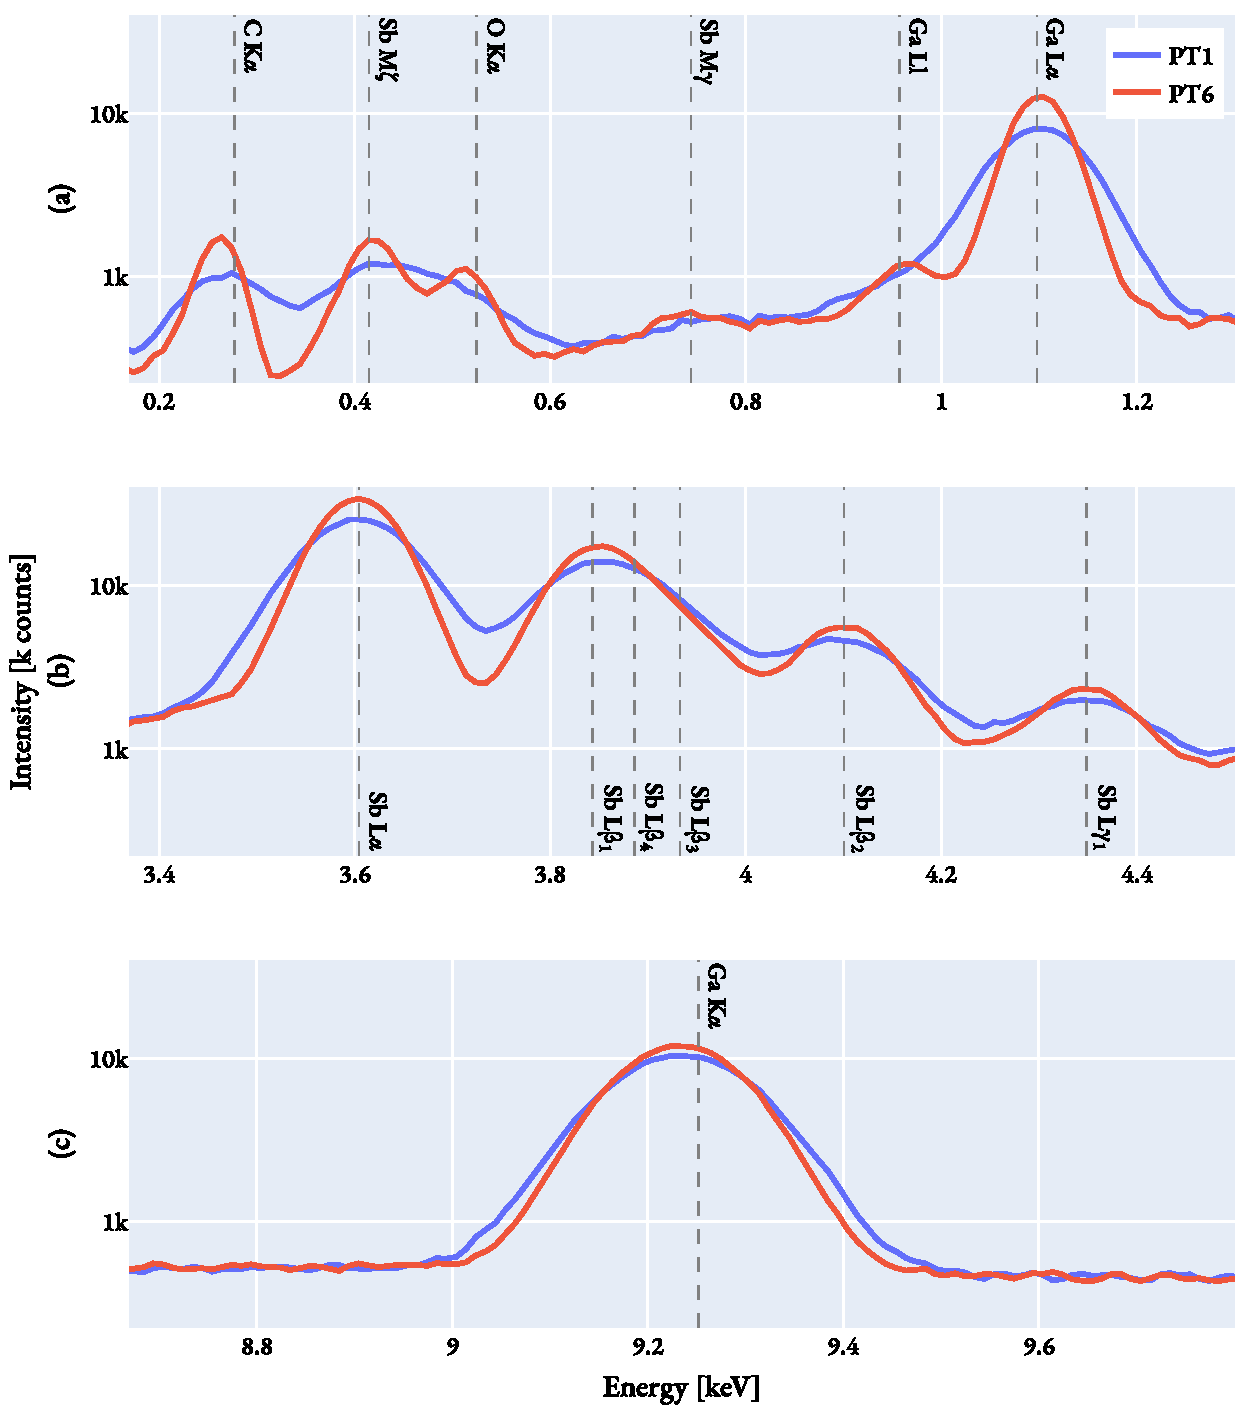
\includegraphics[width=0.95\linewidth]{figures/results/eds_energyResolutions_process_time.pdf}
    \caption{
        Different energy resolutions on the same specimen, because of different process times.
        The maximum (red) and minimum (blue) PT on the instrument is used.
        $E_0 = 30$ kV, $i_b = 50$ pA for both spectra.
        The PT $1$ and PT $4$ spectra are not shown, but are in between the PT $2$ and PT $6$ spectra.
        Panel (a) is the spectrum at low energy, where the effect most influential.
        With PT $1$ the Sb M$\zeta$ and O K$\alpha$ peak are merged, and the Ga L$l$ and Ga L$\alpha$ peaks are merged.
        Panel (b) is the spectrum at medium energy, where the effect less influential, but the peak contrast is lowered.
        Panel (c) is the spectrum at high energy, where the effect is almost negligible.
        All three panels span $1.13$ keV and have the same range of counts.
        The vertical dashed lines are the theoretical line energies.
    }
    \label{fig:results:energy_resolutions_process_time}
\end{figure}


The effect of the process time on the FWHM of the lines is shown in \cref{tab:results:PTvsFWHMs}.
The table shows the measured FWHM of Ga L$\alpha$, Sb L$\alpha$, and Ga K$\alpha$ for different process times.
The measurement is done on the Gaussian fit of the peaks.
Additionally, the FWHM of the Mn K$\alpha$ is estimated for each process time.
The table shows the variations on the GaSb specimen with PT $1$, $2$, $4$, and $6$.
The last row shows the FWHM in the GaAs specimen at PT $6$ for reference.
All spectra in the table were acquired at $30$ kV and $50$ pA.
In the GaSb spectra, the PT $1$ has DT $4$\%, PT $2$ has DT $7$\%, PT $4$ has DT $13$\%, and PT $6$ has DT $44$\%.
The GaAs spectrum with PT $6$ has DT $44$\%.


\begin{table}[phtb]
    \begin{center}
        \caption{
            FWHMs of lines with different process times.
            All the FWHMs are in eV, calculated from the Gaussian fit.
            All spectra are acquired at 30 kV and 50 pA.
            GaSb is used as the specimen, except for the last column, where GaAs is used for reference.
        }
        \renewcommand*{\arraystretch}{1.4}
        \label{tab:results:PTvsFWHMs}
        \begin{tabular}{rrrrrr}
            \hline
            \textbf{Line}       & \textbf{PT 1} & \textbf{PT 2} & \textbf{PT 4} & \textbf{PT 6} & \textbf{PT 6, GaAs} \\
            \hline
            %C K$\alpha$&&&&&\\ % C is not it the models used
            Ga L$\alpha$        & 109           & 88            & 73            & 65            & 67                  \\
            Sb L$\alpha$        & 138           & 122           & 108           & 102           & -                   \\
            Mn K$\alpha$ (est.) & 158           & 143           & 132           & 127           & 129                 \\
            Ga K$\alpha$        & 182           & 172           & 165           & 161           & 163                 \\
            \hline
        \end{tabular}
    \end{center}
\end{table}



\subsection{Beam energy and beam current}
\label{results:beam_energy_and_beam_current}


% comment on (A) and (B)
The energy and the amount of electrons in the probe is important for the emerging X-ray spectrum.
Using a low overvoltage can be problematic.
The green $10$ kV line in \cref{fig:results:GaAs_voltages} has no visible signal from the Ga K$\alpha$ peak, where the overvoltage is around $1.1$.
The overvoltage is also an issue for the Sb L-lines in the $5$ kV spectrum in \cref{fig:results:GaSb_voltages}.
The Sb L-peaks are present, but weak, and the L$l$ peak is not visible.
This issue with the weak Sb-L peaks makes the quantification of Sb difficult at low voltages, as seen further down in \cref{results:initial_quantification}.
The $5$ kV GaAs spectrum is quantified more accurately than the $5$ kV GaSb spectrum.
% because the Ga L$\alpha$ and As L$\alpha$ peaks have similar overvoltages.
In the voltage series, which are group (A) and (B) in \cref{method:acquisition_settings}, the amount of counts in the lower voltages are quite low.
The low amount of counts is due to keeping the beam current constant at $50$ and $25$ pA.
Using a higher beam current on the lower energies would have made normalization more necessary, which is adding a layer of subjective decisions as the spectra must be normalized to something.
% DONE discuss: this might not have been the best choice. For future work one can try to get the same ICR for all voltages, and see if the results are better and still comparable, without normalization.
Even though the $30$ kV spectra in GaAs and GaSb have more counts and are smoother than the other spectra, they both have more artifacts.
% DONE discuss: the amount of artifacts have to be adjusted for the specimen and the goal of the analysis.
% REMOVED: Around 1 keV, the 30 kV and 15 kV spectra are quite similar.
% DONE discuss: at 1 keV, the ionization cross section when using 15 or 30 kV is more or less the same.

% (C) (D) and (E)
As the $30$ and $15$ kV spectra gave better results for GaSb, they were chosen for group (C) and (D).
In (C) different process times were tested, and these results are presented in \cref{results:process_time}.
In (D) different beam currents were tested, while also changing the PT and $E_0$.
% In (E) the data type maps were acquired.
% (D)
The combination of high $i_b$ and high PT in two of the spectra in (D) made the DT very high.
Despite the high DT, the amount of artifacts in the $200$ pA and $400$ pA spectra were similar to the $50$ pA spectra.
However, with DT at $53$\% and $77$\%, the acquisition time was very long.
On the quantification presented in \cref{results:initial_quantification}, the beam energy appears to be more important than the beam current.







\subsection{Duane-Hunt limit}
\label{results:duane_hunt}

The Duane-Hunt limits, or the effective beam energies, are presented in \cref{tab:results:duane_hunt}.
The table shows the Duane-Hunt limit for the $5$, $10$, and $15$ kV spectra.
As the energy range recorded in the spectra were $0-20$ keV, the Duane-Hunt limit of the $30$ kV spectra were not possible to calculate.
All the calculated Duane-Hunt limits are within $0.2$ keV of the nominal beam energy, i.e. the specified beam energy in the SEM software.
The average deviation is $0.06$ keV, with a standard deviation of $0.04$ keV.
This shows that the beam energy is quite stable.
% DONE discuss: the usefulness of calculating the DH limit.





\subsection{Fiori P/B ratio}
\label{results:fiori}

The Fiori numbers are presented in \cref{tab:results:fiori}, with the Fiori P/B ratio in the five rightmost columns.
% # for Ga La, Ga Ka, As La, Sb La, Sb Lb
The ratios are for the Ga L$\alpha$, Ga K$\alpha$, As L$\alpha$, Sb L$\alpha$, and Sb L$\beta$.
The Fiori P/B ratios have a spread between just below $100$ to right under $800$.
The overall highest ratio is for the Ga K$\alpha$ peak in the $30$ kV $25$ pA GaAs spectrum, with a ratio of $770$.
% DONE discuss: repeat why the numbers are so high. That is dividing by one single bg channel, which makes the ratio unaffected by energy resolution.
The equal settings in the GaSb spectrum have a ratio of $408$ for the Ga K$\alpha$ peak.
For the Ga K$\alpha$ peaks, the GaAs spectrum have almost twice as high Fiori P/B ratios as the GaSb spectrum.
The Ga L$\alpha$ peak is present in all the spectra, and it can be used for comparison.
% The background counts around the Ga L$\alpha$ peak is around 2-5 times higher in the GaSb spectra than in the GaAs spectra, which is reflected in the different Fiori ratios for the Ga L$\alpha$ peak.
% DONE sort of discuss: the mu_rho of GaAs is much higher than GaSb above 1 keV because of the double absorption edge. This gives a much higher Fiori ratio for GaAs than GaSb, as the background is lower. But the Ga_La peak ing GaAs is also higher. The specimen dependness is high.
The tabulated data indicate that $E_0$ has the largest impact on the Fiori P/B ratio.
% REMOVED:  The peak height between GaAs and GaSb differs some, but it is probably the background levels which make the biggest impact on the Fiori P/B ratios.
For the Ga L$\alpha$ peak, the Fiori P/B ratios is up to $6$ times higher for GaAs than GaSb.
This shows clearly that the Fiori P/B ratio is specimen dependent, even when using the same peak and setting.



\begin{table}[htbp]
    \begin{center}
        \caption{
            The Duane-Hunt limit in the sub 30 kV spectra.
            All spectra are acquired with PT 6.
        }
        % \renewcommand*{\arraystretch}{1.4}
        \label{tab:results:duane_hunt}
        \begin{tabular}{rrrrr}
            \hline
            \textbf{Group} & \textbf{Specimen} & \textbf{$E_0$} & \textbf{$i_b$} & \textbf{Duane-Hunt limit} \\
            \emph{}        & \emph{}           & \emph{[kV]}    & \emph{[pA]}    & \emph{[kV]}               \\
            \hline
            A              & GaAs              & 5              & 25             & 4.92                      \\
            A              & GaAs              & 10             & 25             & 10.08                     \\
            A              & GaAs              & 15             & 25             & 14.98                     \\
            B              & GaSb              & 5              & 50             & 4.86                      \\
            B              & GaSb              & 10             & 50             & 10.05                     \\
            B              & GaSb              & 15             & 50             & 14.99                     \\
            D              & GaSb              & 15             & 200            & 15.03                     \\
            D              & GaSb              & 15             & 400            & 15.1                      \\
            \hline
        \end{tabular}
    \end{center}
\end{table}

\begin{table}[hbtp]
    \begin{center}
        \caption{
            The Fiori P/B ratios.
            Group A is GaAs, which is sorted by the Ga L$\alpha$ ratio.
            Group B, C, and D is GaSb, which is sorted by the Sb L$\alpha$ ratio.
            The "-" indicates that the line is not present in the spectrum.
        }
        %\renewcommand*{\arraystretch}{1.4}
        \label{tab:results:fiori}
        \begin{tabular}{rrrrrrrrr}
            \hline
            \textbf{Group} & \textbf{$E_0$} & \textbf{$i_b$} & \textbf{PT} & \textbf{Fiori P/B}    & \textbf{Fiori P/B}    & \textbf{Fiori P/B}    & \textbf{Fiori P/B}    & \textbf{Fiori P/B}   \\
            \emph{}        & \emph{[kV]}    & \emph{[pA]}    & \emph{}     & \textbf{Ga L$\alpha$} & \textbf{Ga K$\alpha$} & \textbf{As L$\alpha$} & \textbf{Sb L$\alpha$} & \textbf{Sb L$\beta$} \\
            \hline
            A              & 30             & 50             & 6           & 586                   & 762                   & 236                   & -                     & -                    \\
            A              & 30             & 25             & 6           & 573                   & 770                   & 233                   & -                     & -                    \\
            A              & 15             & 25             & 6           & 414                   & 187                   & 250                   & -                     & -                    \\
            A              & 10             & 25             & 6           & 280                   & 0                     & 206                   & -                     & -                    \\
            A              & 5              & 25             & 6           & 155                   & -                     & 140                   & -                     & -                    \\
            \hline
            C              & 30             & 50             & 4           & 87                    & 407                   & -                     & 386                   & 169                  \\
            C              & 30             & 50             & 2           & 84                    & 414                   & -                     & 386                   & 169                  \\
            C              & 30             & 50             & 1           & 83                    & 414                   & -                     & 386                   & 168                  \\
            B              & 30             & 50             & 6           & 86                    & 408                   & -                     & 385                   & 168                  \\
            D              & 30             & 400            & 1           & 86                    & 320                   & -                     & 360                   & 156                  \\
            B              & 15             & 50             & 6           & 110                   & 138                   & -                     & 215                   & 97                   \\
            D              & 15             & 200            & 6           & 109                   & 131                   & -                     & 214                   & 97                   \\
            D              & 15             & 400            & 6           & 107                   & 124                   & -                     & 211                   & 95                   \\
            B              & 10             & 50             & 6           & 113                   & 9                     & -                     & 140                   & 65                   \\
            B              & 5              & 50             & 6           & 91                    & -                     & -                     & 16                    & 5                    \\
            \hline
        \end{tabular}
    \end{center}
\end{table}



% \subsection{Portion of counts in the peaks}
% \label{results:portion_of_counts}

% \brynjar{Something about the portion of counts in the peaks vs. in the background.}





\clearpage


\subsection{Summarization of the performance parameters}
\label{results:summarization_of_the_performance_parameters}

% \brynjar{DONE: add table and description of the summary for the performance parameters.}

This last section in the performance parameters contains a summarization of the parameters for the detector and the acquisition parameters.
\cref{tab:results:performance_summary} gives the values for the parameters with a comment.
The energy resolution of the detector used in this work is $127 \pm6$ eV at ICR between $1$ k and $42$ k cps, with the highest PT avaliable.
The energy axis of the instrument is calibrated well, with low deviations between the specified scale and offset, and their calibrated values.
This is strengthened by the low deviation in calibrated peak positions.
The Duane-Hunt limits are all close to the nominal beam energy.
The Fiori P/B ratios acquired were at the highest $770$ for GaAs and $410$ for GaSb.

\begin{table}[hbpt]
    \begin{center}
        \caption{
            A summary of the performance parameter results.
            %
            %
        }
        \renewcommand*{\arraystretch}{1.2}
        \label{tab:results:performance_summary}
        \begin{tabular}{p{2.5cm}p{4cm}p{7cm}}
            \hline
            \textbf{Parameter}                                            & \textbf{Value}                 & \textbf{Comment}                                                                                                                                                                                       \\
            \hline%%%%%%
            \hyperref[results:duane_hunt]{Duane-Hunt limit}               & $E_0 \pm 0.2$ keV              & For the detector. Average deviation was $0.06 \pm0.04$ keV, but the value specified include the maximum deviations.                                                                                    \\
            \hyperref[results:energy_resolution]{Energy resolution}       & $127 \pm6$ eV                  & Parameter for the detector, but highly dependent on PT. Recorded at the highest PT on GaAs and GaSb. The variation is from different reference peaks in the calculation and different $E_0$ and $i_b$. \\
            \hyperref[results:scaleoffset]{Scale}                         & $10.007 \pm0.038$ eV           & For the detector. The scale of the GaAs spectra varied slightly more than the GaSb spectra.                                                                                                            \\
            \hyperref[results:scaleoffset]{Offset}                        & $- 0.205 \pm0.004$ keV         & For the detector.                                                                                                                                                                                      \\
            \hyperref[results:scaleoffset]{Deviations in peak positions}  & $0-2$ eV                       & For the detector.                                                                                                                                                                                      \\
            \hyperref[results:fiori]{Fiori P/B ratio}                     & $770$ for Ga K$\alpha$ in GaAs & For the detector, acquisition parameters and specimen dependent. The value is the highest achieved.                                                                                                    \\
            \hyperref[results:fiori]{Fiori P/B ratio}                     & $410$ for Ga K$\alpha$ in GaSb & "                                                                                                                                                                                                      \\
            \hyperref[results:peak_ratios]{Peak ratios}                   & GaSb > GaAs and $\propto E_0$  & Varying with acquisition parameters and specimen.                                                                                                                                                      \\
            \hline%%%%%%
            \hyperref[results:beam_energy_and_beam_current]{Beam energy}  & $15$ kV or $30$ kV             & Best results were acquired with higher beam energy.                                                                                                                                                    \\
            \hyperref[results:beam_energy_and_beam_current]{Beam current} & Not a specific number          & Dependent on $E_0$, and needs to give enough counts.                                                                                                                                                   \\
            \hyperref[results:process_time]{Process time}                 & Not a number                   & Should be high, but the highest give long acquisition time.                                                                                                                                            \\
            \hline
        \end{tabular}
    \end{center}
\end{table}
}


\clearpage

















% 4.4
\section{Quantitative analysis}
\label{results:quantitative}

% DONE say that the average, >10%, and <5% are in tables here, while all the compositions are in the appendix.
This section presents the results from the quantitative analysis, using different correction methods.
With $15$ spectra analyzed, the tables are large and thus average values from different methods are used to give an overview of the results.
The results from all $15$ spectra in the initial quantification are shown in \cref{results:initial_quantification}.
For this and the remaining methods, a table with the average values, deviations above $10$ at.\%, and deviations below $5$ at.\% are shown.
The $5$ kV GaSb spectrum is excluded from these average tables, as the spectrum had several issues.
The full tables with quantification using the thin film assumption, the ZAF absorption correction, and corrections with PAP are given in \hyperref[appendix:tables]{Appendix C}.


\subsection{Initial quantification}
\label{results:initial_quantification}

% initial quantification (AZtec and i/i_sum)
Initial quantification was done with the AZtec software and with the uncorrected intensity ratio method.
The intensity ratio method is calculated with \cref{eq:theory:quantitative:area_ratio}, and it gives relative compositions as described in \cref{theory:quantitative:principle}.
AZtec too gives relative compositions, based on the elements confirmed to be present in the spectrum.
Average values for the initial quantification results are shown in \cref{tab:results:initial_quantification_stats}.
Results from all the $15$ spectra are shown in \cref{tab:results:initial_quantification}, and plotted in \cref{fig:results:initial_quantification}.
% \ton{I decided to round the percentages to integers. OK?} Ok
As the table and figure show, some results are close to $50$ at.\%.
% DONE discuss: "Ton: Statement/observation OK, but in discussion: this is not proof for accuracy, it could be a coincident, have to consider error range. But here keep figure and comment as is"
The summary table also show that on average GaSb is quantified closer to $50$ at.\% than GaAs.
All AZtec results are with the SEM EDS setting, if not stated otherwise.
In $12$ of the $15$ spectra, AZtec gives a result at $50\pm2$ at.\%.
$2$ of spectra are quantified at $50\pm4$ at.\%.
The $5$ kV GaSb spectrum is quantified at 39:61, which is the most deviating result from AZtec.
The $5$ intensity ratios from GaSb spectra with $E_0 = 30$ kV are at $50\pm2$ at.\%.
The three $15$ kV results from GaSb have a deviation of $\pm10$ at.\%, which show the need for closer inspection.
The remaining results are also in need of closer inspections, as the results from the uncorrected intensity ratio method give high deviations.
% The low energy results from GaAs have a high deviation, probably due to issues with overvoltage.


\begin{table}[phtb]
    \begin{center}
        \caption{
            Numbers for the at\% deviations in the initial quantification, see \cref{tab:results:initial_quantification}
            The GaSb 5 kV spectrum is excluded from the numbers, as it is viewed as an outlier.
            The table gives the average deviation in at\% from 50 at\%, for GaAs and GaSb seperated.
            The number of deviations below 5 at\% and above 10 at\% are also tabulated.
        }
        %\renewcommand*{\arraystretch}{1.4}
        \label{tab:results:initial_quantification_stats}
        \begin{tabular}{rrrr}
            \hline
            \textbf{Specimen} & \textbf{Number}         & \textbf{AZtec} & \textbf{Intensity ratio} \\
            \hline
            GaAs              & Average deviation, at\% & 2 at\%         & 12 at\%                  \\
                              & Deviations $>10$ at\%   & 0              & 4                        \\
                              & Deviations  $<5$  at\%  & 5              & 0                        \\
            \hline
            GaSb              & Average deviation, at\% & 1 at\%         & 6 at\%                   \\
                              & Deviations $>10$ at\%   & 0              & 1                        \\
                              & Deviations  $<5$  at\%  & 9              & 5                        \\

            \hline
        \end{tabular}
    \end{center}
\end{table}

\newgeometry{top=2cm} % change the margins to fit the table.

\begin{table}[phtb]
    \begin{center}
        \caption{
            Initial quantification in selected spectra.
            Compositions from AZtec and the intensity ratio method.
            Each spectrum corresponds to two lines, one for each element.
            The table is summarized in \cref{tab:results:initial_quantification_stats}.
        }
        %\renewcommand*{\arraystretch}{1.4}
        \label{tab:results:initial_quantification}
        \begin{tabular}{rrrrrrrr}
            \hline
            \textbf{ Group} & \textbf{Line} & \textbf{$E_0$} & \textbf{$i_b$} & \textbf{PT} & \textbf{Intensity} & \textbf{AZtec comp.} & \textbf{Intensity ratio comp.} \\
            \emph{}         & \emph{}       & \emph{[kV]}    & \emph{[pA]}    & \emph{}     & \emph{[k counts]}  & \emph{at\%}          & \emph{at\%}                    \\
            \hline
            A               & As L$\alpha$  & 5              & 25             & 6           & 13                 & 53                   & 43                             \\
            A               & Ga L$\alpha$  & 5              & 25             & 6           & 16                 & 47                   & 57                             \\
            A               & As L$\alpha$  & 10             & 25             & 6           & 37                 & 52                   & 40                             \\
            A               & Ga L$\alpha$  & 10             & 25             & 6           & 51                 & 48                   & 60                             \\
            A               & As L$\alpha$  & 15             & 25             & 6           & 62                 & 51                   & 36                             \\
            A               & Ga L$\alpha$  & 15             & 25             & 6           & 103                & 49                   & 64                             \\
            A               & As K$\alpha$  & 30             & 25             & 6           & 84                 & 48                   & 36                             \\
            A               & Ga K$\alpha$  & 30             & 25             & 6           & 141                & 52                   & 64                             \\
            A               & As K$\alpha$  & 30             & 50             & 6           & 180                & 48                   & 36                             \\
            A               & Ga K$\alpha$  & 30             & 50             & 6           & 303                & 52                   & 64                             \\
            \hline
            B               & Ga L$\alpha$  & 5              & 50             & 6           & 19                 & 39                   & 97                             \\
            B               & Sb L$\alpha$  & 5              & 50             & 6           & 1                  & 61                   & 3                              \\
            B               & Ga L$\alpha$  & 10             & 50             & 6           & 46                 & 47                   & 75                             \\
            B               & Sb L$\alpha$  & 10             & 50             & 6           & 27                 & 53                   & 25                             \\
            B               & Ga L$\alpha$  & 15             & 50             & 6           & 74                 & 49                   & 58                             \\
            B               & Sb L$\alpha$  & 15             & 50             & 6           & 94                 & 51                   & 42                             \\
            B               & Ga K$\alpha$  & 30             & 50             & 6           & 191                & 50                   & 48                             \\
            B               & Sb L$\alpha$  & 30             & 50             & 6           & 359                & 50                   & 52                             \\
            \hline
            C               & Ga K$\alpha$  & 30             & 50             & 4           & 189                & 50                   & 48                             \\
            C               & Sb L$\alpha$  & 30             & 50             & 4           & 350                & 50                   & 52                             \\
            C               & Ga K$\alpha$  & 30             & 50             & 2           & 184                & 50                   & 49                             \\
            C               & Sb L$\alpha$  & 30             & 50             & 2           & 330                & 50                   & 51                             \\
            C               & Ga K$\alpha$  & 30             & 50             & 1           & 178                & 50                   & 51                             \\
            C               & Sb L$\alpha$  & 30             & 50             & 1           & 304                & 50                   & 49                             \\
            \hline
            D               & Ga L$\alpha$  & 15             & 200            & 6           & 155                & 49                   & 57                             \\
            D               & Sb L$\alpha$  & 15             & 200            & 6           & 200                & 51                   & 43                             \\
            D               & Ga L$\alpha$  & 15             & 400            & 6           & 284                & 49                   & 57                             \\
            D               & Sb L$\alpha$  & 15             & 400            & 6           & 367                & 51                   & 43                             \\
            D               & Ga K$\alpha$  & 30             & 400            & 1           & 1724               & 50                   & 50                             \\
            D               & Sb L$\alpha$  & 30             & 400            & 1           & 2996               & 50                   & 50                             \\
            %
            %E&Map&&&&&&\\
            %E&Map&&&&&&\\
            %&&&&&&&\\
            \hline
        \end{tabular}
    \end{center}
\end{table}
\restoregeometry % put the margins back to normal


% figures/results/initial_quantification.pdf
\begin{figure}[htbp]
    \centering
    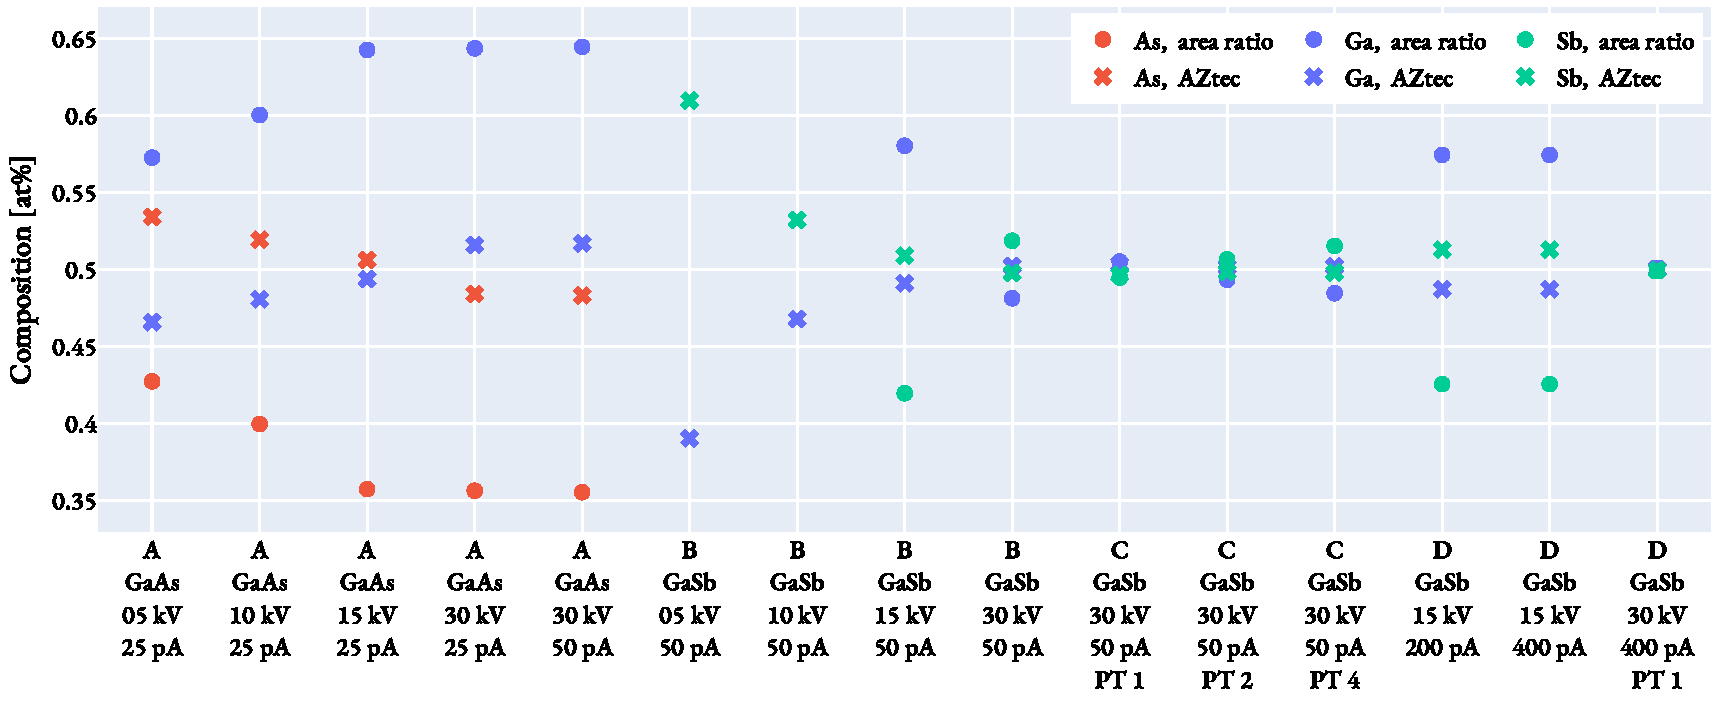
\includegraphics[width=0.99\linewidth]{figures/results/initial_quantification.pdf}
    \caption{
        Initial quantification results in at.\%.
        The X markers are the quantification from AZtec.
        The circle markers are the quantification from the intensity ratio, without corrections.
        The group, specimen, $E_0$, $i_b$, and PT are shown on the x-axis.
        The spectra without noted PT are taken with PT $6$.
        The same data is tabulated in \cref{tab:results:initial_quantification}.
    }
    \label{fig:results:initial_quantification}
\end{figure}








% \subsection{Quantification of SEM EDS data based on the Cliff-Lorimer method} % Tons suggested title
\subsection{Quantification of SEM EDS data with the thin film approximation}
\label{results:quantification_cliff_lorimer}


Quantitative analysis of the SEM EDS bulk spectra was also done under the presumption that the specimen was a TEM specimen, i.e. under the thin film approximation.
The thin film approximation assumes no absorption of the created X-rays in the specimen, and is a part of the Cliff-Lorimer (CL) method covered in \cref{sec:theory:quantitative:k_factor_vs_k_ratio}.
The presumption that the specimen is a TEM specimen was both applied in AZtec with the "TEM setting", and in HyperSpy with the CL method.
TEM EDS quantification of SEM EDS data can readily be done, even though it is formally incorrect.

% the table
The results from the TEM EDS quantification routines are tabulated in \hyperref[appendix:tables]{Appendix C} in \cref{tab:results:TEM_quantification}, and average numbers from that table is presented in \cref{tab:results:TEM_quantification_stats}.
% TODO: check the appendix reference
The calculated k-factors, which are extracted from AZtec and needed for the CL method in HyperSpy, are included in \cref{tab:results:TEM_quantification}.
The CL method in HyperSpy was done with and without the TEM absorption corrections, which is a part of the implemented CL quantification function.
The "CL*" column is without absorption corrections, and the other "CL" columns are with the TEM absorption corrections, where the $t$ is the set specimen thickness.
Six $t$ values are: $50$ nm, $100$ nm, $200$ nm, $400$ nm, $1000$ nm, and $10000$ nm.
% DONE discuss: compare t with penetration depth, and argument for the very high maximum tested.


% comment on the severely poor results from GaAs at 5 kV
The GaSb spectrum at $5$ kV is poorly quantified by AZtec.
AZtec is quantifying the $5$ kV GaSb spectrum with the Ga L$\alpha$ and Sb M$\zeta$ peaks.
Sb M$\zeta$ is around $0.4$ keV, and at such low energy the matrix absorption is high, and the resulting composition is $91:9$.
% DONE discuss: even thought the detector is with a polymer (?) window for allowing low energy X-rays, the absorption is still high in the specimen (the window let the X-rays pass, but few are coming.)
The Sb M$\zeta$ peak is not available in HyperSpy, and no k-factor is given for the Sb L$\alpha$ line in this spectrum.
Thus, it is not possible to quantify the $5$ kV GaSb spectrum with HyperSpy.
% When using TEM mode, AZtec selects the Sb M$\zeta$ line at 5 kV, and as this line is not included in HyperSpy, the 5 kV GaSb spectra were not quantified in HyperSpy.
% DONE discuss: not possible to quantify with HyperSpy at 5 kV, as the Sb M$\zeta$ line is missing and thus there are no k-factor for Sb La.
% DONE discuss: HyperSpy will not give k-factors, even though some people ask for it (Gitter). This is becaues that would give a high uncertainty, as the k-factors are partly dependent on the detector.
% DONE discuss from Ton: "In discussion can debate of other more correct k-factors would lead to substantial better quantification or that own k-factors can be extracted from the data you have and if that helps, even seen the wrong preassumption"


% comment on the table values
The TEM EDS quantification results of the SEM EDS data are in general deviating from the reference value of $50:50$.
Opposite to the SEM EDS quantification setting in AZtec, the GaAs spectra are quantified closer to the reference value than the GaSb spectra.
The "TEM EDS setting" AZtec results are deviating much more from $50:50$ compared to the AZtec results using the "SEM EDS setting", presented in \cref{results:initial_quantification}.
% The average numbers for \cref{tab:results:TEM_quantification} in \cref{tab:results:TEM_quantification_stats} are calculated without the 5 kV GaSb spectra, as the 5 kV spectra were not quantified in HyperSpy.
% DONE discuss: this celarly show that AZtec is doing different quant with SEM and TEM, but the difference is not in the documentation. We know they do XPP from the blog post, and that could have been stated in the manual.
The CL quantification without absorption corrections perform similar to AZtec, and the deviations are improved for the CL quantifications with absorption corrections, where $t$ is set to $50$, $100$, $200$, and $400$ nm.
% DONE discuss: HyperSpy is actually better than AZtec, on TEM setting. Also, it is a special case, other specimen might have very different results.
The CL quantification with $t$ is set to $200$ nm gives better results than the uncorrected intensity ratio method, but still at an average deviation of $5$ at.\% from the reference value for GaAs and GaSb.
% DONE discuss: why are these t-values good? compare to the range r, and comment that the increasing devaition with high t can be due to ...?
When $t$ is set to $1000$ nm, the average deviations increase from $400$ nm, and $4$ of the GaSb spectra are quantified at $> 10$ at.\% deviation, illustrating some issue with high $t$.
The deviations are increased further when $t$ is set to $10000$ nm.
% DONE discuss: in general, the TEM results are poor, especially true for the AZtec results. The CL with absorption corrections show that absorption corrections can improve the results, but using TEM routines on SEM data is not recommended. Setting the best t is also not trivial.
% DONE discuss: To conclude, the TEM EDS quantification of SEM EDS data show that the routines are built on similar principles, but that the routines have differences which are important. Too unrelibale!

% DONE discuss from Ton: "What is the take-home message? (TEM approach on SEM EDS, not works well, can get some improvement in right direction by adding corrections?)" -> TEM quant with corrections can work, but what corrections should be used? Too unreliable.

\begin{table}[phtb]
    \begin{center}
        \caption{
            Numbers for the at\% deviations with the thin film assumption, i.e. the TEM quantification routines.
            The table is a summary of \cref{tab:results:TEM_quantification}.
            The AZtec result is from the "TEM EDS setting", and the CL results are from the Cliff-Lorimer method in HyperSpy.
            CL* is without corrections, the others CL have absorption correction with input thicknesses $t$, in nm.
        }
        %\renewcommand*{\arraystretch}{1.4}
        \label{tab:results:TEM_quantification_stats}
        \begin{tabular}{rrrrrrrrrr}
            \hline
            \textbf{Specimen} & \textbf{Number}         & \textbf{AZtec} & \textbf{CL*} & \textbf{CL}   & \textbf{CL}    & \textbf{CL}    & \textbf{CL}    & \textbf{CL}   & \textbf{CL}    \\
            \emph{}           & \emph{}                 & \emph{TEM}        & \emph{}      & \emph{$t$=50} & \emph{$t$=100} & \emph{$t$=200} & \emph{$t$=400} & \emph{$t$=1k} & \emph{$t$=10k} \\
            \hline
            GaAs              & Average deviation, at\% & 8 at\%         & 9 at\%       & 8 at\%        & 7 at\%         & 5 at\%         & 5 at\%         & 7 at\%        & 6 at\%         \\
                              & Deviations $>10$ at\%   & 1              & 1            & 1             & 0              & 0              & 0              & 0             & 2              \\
                              & Deviations  $<5$  at\%  & 1              & 1            & 1             & 1              & 2              & 3              & 1             & 2              \\
            \hline
            GaSb              & Average deviation, at\% & 11 at\%        & 9 at\%       & 8 at\%        & 7 at\%         & 5 at\%         & 7 at\%         & 11 at\%       & 21 at\%        \\
                              & Deviations $>10$ at\%   & 3              & 3            & 0             & 0              & 1              & 1              & 4             & 9              \\
                              & Deviations  $<5$  at\%  & 0              & 1            & 0             & 0              & 3              & 1              & 5             & 0              \\
            \hline
        \end{tabular}
    \end{center}
\end{table}












\clearpage


\subsection{ZAF absorption corrections}
\label{results:ZAF}

The ZAF absorption corrections were done with \cref{eq:theory:quantitative:absorption}.
The calculated maximum electron range $r$ is presented in \cref{tab:results:ZAF_corrections_range_r}.
To calculate the absorption correction factors, $r$ is divided by $2$, $3$, and $4$ to get different approximations for the average depth of origin of the X-rays.
The calculated ZAF absorption correction factors are given in \cref{tab:results:ZAF_corrections_factors}, which are applied to get compositions in \cref{tab:results:ZAF_corrections_compositions}, which are presented with average numbers in \cref{tab:results:ZAF_corrections_compositions_stats}.


% comment on the table values
The ZAF absorption corrections improve the GaAs quantification, but deviations from $50$ at.\% in the GaSb quantification is increased.
For GaAs, the best result is achieved when the maximum electron range is divided by $4$, i.e. the absorption correction is applied to an average point close to the surface.
% DONE? illustrate the different r values? Also, r is different for kV values.
When $r$ is divided by four, the average deviation is improved from $12$ at.\% to $7$ at.\%, compared to the uncorrected intensity ratio method.
With $r/4$, the number of spectra with $> 10$ at.\% deviation is reduced from $4$ to $2$, and the number of spectra with $< 5$ at.\% deviation is increased from $0$ to $3$.
For GaSb, the average deviation decrease when $r$ is divided by a higher number, but the deviations are $> 20$ at.\% anyway, which is quite poor.
% DONE discuss: ZAF A implies that GaAs needs abs. corr, but that GaSb have issue with something else. Z is close for Ga and As, while far apart for Ga Sb. Thus, Z effects might not be negligible as stated in Goldstein.

\begin{table}[phtb]
    \begin{center}
        \caption{
            Numbers for the at\% deviations from $50:50$ in the ZAF absorption corrections, in \cref{tab:results:ZAF_corrections_compositions}.
            The table gives the average and the number of deviations below 5 at\% and above 10 at\% are counted, for GaAs and GaSb separated.
            %
        }
        %\renewcommand*{\arraystretch}{1.4}
        \label{tab:results:ZAF_corrections_compositions_stats}
        \begin{tabular}{rrrrrr}
            \hline
            \textbf{Specimen} & \textbf{Numbers}        & \textbf{Uncorr.} & \textbf{ZAF A, r/2} & \textbf{ZAF A, r/3} & \textbf{ZAF A, r/4} \\
            \hline

            %GaAs&&&&&\\
            GaAs              & Average deviation, at\% & 12 at\%          & 11 at\%             & 8 at\%              & 7 at\%              \\
                              & Deviations $>10$ at\%   & 4                & 3                   & 2                   & 2                   \\
                              & Deviations  $<5$  at\%  & 0                & 1                   & 2                   & 3                   \\
            \hline
            %GaSb&&&&&\\
            GaSb              & Average deviation, at\% & 6 at\%           & 30 at\%             & 25 at\%             & 21 at\%             \\
                              & Deviations $>10$ at\%   & 1                & 9                   & 9                   & 6                   \\
                              & Deviations  $<5$  at\%  & 5                & 0                   & 0                   & 0                   \\

            \hline
        \end{tabular}
    \end{center}
\end{table}






\subsection{XPP corrections}
\label{results:XPP}

The XPP corrections were done in two ways, where the measured intensity of a peak $I_A$ is divided by the calculated generated intensity of the peak $F$, or by the calculated XPP absorption correction factor $f(\chi)$.
% DONE disucss: divide by F is a Z correction, and divide by f(chi) is both Z and A correction.
Both ways are presented in \cref{tab:results:XPP_compositions}, where the uncorrected compositions are included for comparison.
% All compositions are in atomic percent, and are calculated with the relative peak area method.
Average numbers for the XPP corrections are given in \cref{tab:results:XPP_compositions_stats}.
$F$ and $f(\chi)$ are calculated with the XPP notebook, and are dependent on $E_0$, $E_C$ of the line, and the elements with their weight fraction of the elements.
The elements and their weight fractions are used to calculate the density $\rho$, the mean atomic mass $M$, the mean ionization potential $J$, the mean atomic number $\bar{Z}$, the backscattering coefficient $R$, and $\mu_\rho$ of the line at $E_0$.
The weight fractions used in the calculations are set to the equivalent of a $50:50$ atomic percent composition, as this should give the best possible correction factors.
A finished product for XPP bulk corrections should have iterative calculations of the weight fractions, but these results are aiming to demonstrate the possible usefulness of XPP corrections, thus the best available input parameters are used.


The corrections with $f(\chi)$, i.e. the absorption correction, improves the GaAs quantification.
Similar to the ZAF absorption corrections, the GaSb quantification is not improved when corrected with $f(\chi)$.
The absorption correction with XPP reduce the average deviation in GaAs from $12$ at.\% to $5$ at.\%, which is better than the ZAF absorption correction.
% DONE discuss: again, the GaSb is made much worse. Doing abs. corr if not needed seems to make the results bad, at lest with the avaliable input parameters used in this work.

When GaSb is corrected with $F$, the average is unchanged.
However, in the uncorrected quantification, the $30$ kV GaSb spectra are quantified very close to the reference value, and the $F$ correction makes these $30$ kV spectra deviate more.
The quantification of the $15$ kV and $10$ kV GaSb spectra are improved with the $F$ correction, which is why the average is unchanged.
In the $30$ kV spectra, the Ga line is given a weight which increase its composition relative to the Sb line, while the opposite is done in the $15$ kV and $10$ kV spectra.
The XPP corrections are dependent on the beam energy, making the effect at $30$ kV different from the effect at $15$ kV and $10$ kV.


% \newgeometry{top=2cm} % change the margins to fit the table.
\begin{table}[phtb]
    \begin{center}
        \caption{
            Compositions from the area ratio method XPP corrections.
            Two type of corrections have been tested where the measured intensity $I_A$ of each peak have been divided by (1) the peaks absorption correction factor $f(\chi)$, and (2) by the peaks area $F$ of the $\phi(\rho z)$ curve.
            $f(\chi)$ is defined in \cref{eq:theory:quantitative:pap:absorption_correction}, and $F$ is defined in \cref{eq:theory:quantitative:pap:general_principle:F}.
        }
        %\renewcommand*{\arraystretch}{1.4}
        \label{tab:results:XPP_compositions}
        \begin{tabular}{rrrrrrrr}
            \hline
            \textbf{Groups} & \textbf{Line} & \textbf{$E_0$} & \textbf{$i_b$} & \textbf{Uncorr. area ratio} & \textbf{XPP corr. $(I_A/f(\chi))$} & \textbf{XPP corr. $(I_A/F)$} \\
            \emph{}         & \emph{}       & \emph{[kV]}    & \emph{[pA]}    & \emph{[at\%]}               & \emph{[at\%]}                      & \emph{[at\%]}                \\
            \hline
            A               & As L$\alpha$  & 5              & 25             & 43                          & 43                                 & 44                           \\
            A               & Ga L$\alpha$  & 5              & 25             & 57                          & 57                                 & 56                           \\
            A               & As L$\alpha$  & 10             & 25             & 40                          & 42                                 & 41                           \\
            A               & Ga L$\alpha$  & 10             & 25             & 60                          & 58                                 & 59                           \\
            A               & As L$\alpha$  & 15             & 25             & 36                          & 39                                 & 36                           \\
            A               & Ga L$\alpha$  & 15             & 25             & 64                          & 61                                 & 64                           \\
            A               & As K$\alpha$  & 30             & 25             & 36                          & 36                                 & 37                           \\
            A               & Ga K$\alpha$  & 30             & 25             & 64                          & 64                                 & 63                           \\
            A               & As K$\alpha$  & 30             & 50             & 36                          & 36                                 & 37                           \\
            A               & Ga K$\alpha$  & 30             & 50             & 64                          & 64                                 & 63                           \\
            \hline
            B               & Ga L$\alpha$  & 5              & 50             & 97                          & 97                                 & 91                           \\
            B               & Sb L$\alpha$  & 5              & 50             & 3                           & 3                                  & 9                            \\
            B               & Ga L$\alpha$  & 10             & 50             & 75                          & 79                                 & 65                           \\
            B               & Sb L$\alpha$  & 10             & 50             & 25                          & 21                                 & 35                           \\
            B               & Ga L$\alpha$  & 15             & 50             & 58                          & 67                                 & 50                           \\
            B               & Sb L$\alpha$  & 15             & 50             & 42                          & 33                                 & 50                           \\
            B               & Ga K$\alpha$  & 30             & 50             & 48                          & 48                                 & 56                           \\
            B               & Sb L$\alpha$  & 30             & 50             & 52                          & 52                                 & 44                           \\
            \hline
            C               & Ga K$\alpha$  & 30             & 50             & 48                          & 48                                 & 56                           \\
            C               & Sb L$\alpha$  & 30             & 50             & 52                          & 52                                 & 44                           \\
            C               & Ga K$\alpha$  & 30             & 50             & 49                          & 49                                 & 57                           \\
            C               & Sb L$\alpha$  & 30             & 50             & 51                          & 51                                 & 43                           \\
            C               & Ga K$\alpha$  & 30             & 50             & 51                          & 50                                 & 58                           \\
            C               & Sb L$\alpha$  & 30             & 50             & 49                          & 50                                 & 42                           \\
            \hline
            D               & Ga K$\alpha$  & 30             & 400            & 50                          & 50                                 & 58                           \\
            D               & Sb L$\alpha$  & 30             & 400            & 50                          & 50                                 & 42                           \\
            D               & Ga L$\alpha$  & 15             & 200            & 57                          & 66                                 & 49                           \\
            D               & Sb L$\alpha$  & 15             & 200            & 43                          & 34                                 & 51                           \\
            D               & Ga L$\alpha$  & 15             & 400            & 57                          & 66                                 & 49                           \\
            D               & Sb L$\alpha$  & 15             & 400            & 43                          & 34                                 & 51                           \\
            \hline
        \end{tabular}
    \end{center}
\end{table}
\restoregeometry % put the margins back to normal
 % Is now in the appendix
\begin{table}[phtb]
    \begin{center}
        \caption{
            Numbers for the XPP corrected compositions listed in \cref{tab:results:XPP_compositions}.
            The XPP corrections are done in two ways.
            The uncorrected intensity ratio results are listed for reference.
            % The table gives the average and the number of deviations below 5 at\% and above 10 at\% are counted, for GaAs and GaSb separated.
            $f(\chi)$ the absorption correction, and $F$ is the generated amount of X-rays, i.e. Z corrections.
            $f(\chi)$ is defined in \cref{eq:theory:quantitative:pap:absorption_correction}, and $F$ is defined in \cref{eq:theory:quantitative:pap:general_principle:F}.
        }
        %\renewcommand*{\arraystretch}{1.4}
        \label{tab:results:XPP_compositions_stats}
        \begin{tabular}{rrrrr}
            \hline
            \textbf{Specimen} & \textbf{Number}         & \textbf{Uncorr.} & \textbf{XPP corr. $(I_A/f(\chi))$} & \textbf{XPP corr. $(I_A/F)$} \\
            %
            \hline

            GaAs              & Average deviation, at\% & 12 at\%          & 5 at\%                             & 11 at\%                      \\
                              & Deviations $>10$ at\%   & 4                & 0                                  & 3                            \\
                              & Deviations  $<5$  at\%  & 0                & 2                                  & 0                            \\
            \hline

            GaSb              & Average deviation, at\% & 6 at\%           & 38 at\%                            & 6 at\%                       \\
                              & Deviations $>10$ at\%   & 1                & 9                                  & 1                            \\
                              & Deviations  $<5$  at\%  & 5                & 0                                  & 3                            \\

            \hline
        \end{tabular}
    \end{center}
\end{table}















\subsection{Summary of the quantification results}
\label{results:quantification_summary}

The results presented in this section show quantifaction from: AZtec, uncorrected intensities, ZAF absorption corrections, and two XPP corrections.
With $50:50$ atomic weight as the reference goal, the results from AZtec are the closest.
The corrections applied to the intensities push the results both towards and away from the reference value, depending on the specimen and the beam energy.
The GaAs spectra are quantified closer to the reference value when corrected with absorption corrections, and correction with $f(\chi)$ from the XPP model gave an average deviation of $5$ at.\%.
The GaSb spectra are quantified closer to the reference value when corrected with $F$ from the XPP model, with an average deviation of $6$ at.\%.